\pdfminorversion=4
\documentclass[]{article}

%%%%%%%%%%%%%%%%%%%
% Packages/Macros %
%%%%%%%%%%%%%%%%%%%
\usepackage{amssymb,latexsym,amsmath}     % Standard packages
\usepackage{graphicx}
\graphicspath{ {./images/} }


%%%%%%%%%%%
% Margins %
%%%%%%%%%%%
\addtolength{\textwidth}{1.0in}
\addtolength{\textheight}{1.00in}
\addtolength{\evensidemargin}{-0.75in}
\addtolength{\oddsidemargin}{-0.75in}
\addtolength{\topmargin}{-.50in}


%%%%%%%%%%%%%%%%%%%%%%%%%%%%%%
% Theorem/Proof Environments %
%%%%%%%%%%%%%%%%%%%%%%%%%%%%%%
\newtheorem{theorem}{Theorem}
\newenvironment{proof}{\noindent{\bf Proof:}}{$\hfill \Box$ \vspace{10pt}}


%%%%%%%%%%%%
% Document %
%%%%%%%%%%%%
\begin{document}

\title{HW5}
\author{Amitesh Badkul}
\maketitle

\begin{abstract}
This document contains my attempt at the homework 5 problems of the course
Learning From Data ({\bf CS156}) as taught by Professor {\em Yaser Abu-Mostafa, Caltech}.
\end{abstract}


%%%%%%%%%%%%%%%
\begin{enumerate}
\item[$\bullet$] {\bf Linear Regression}
    \begin{enumerate}
        \subitem {\small 1.[c], Using the given equation the answer can be obtained}
    \end{enumerate}

\item[$\bullet$] {\bf Non Linear Transform}
    \begin{enumerate}
        \subitem {\small 2.[d], the $x_1$ should be negative and $x_2$ should be positive to acheive the given graph}
\includegraphics{hyperbola}
        \subitem {\small 3.[c], The VC Dimensions of the above equation is $13$}
    \end{enumerate}


\item[$\bullet$] {\bf Gradient Descent}
    \begin{enumerate}
        \subitem {\small 4.[e], self-explainatory}
        \subitem {\small 5.[d], a program gives the number of iterations as $10$, the  program calculates the gradient of the error function and tries to acheive a minima }
        \subitem {\small 6.[e], check the output for the written code}
        \subitem {\small 7.[a], An inefficent method for reaching the minima}
    \end{enumerate}

\item[$\bullet$] {\bf Logistic Regression}
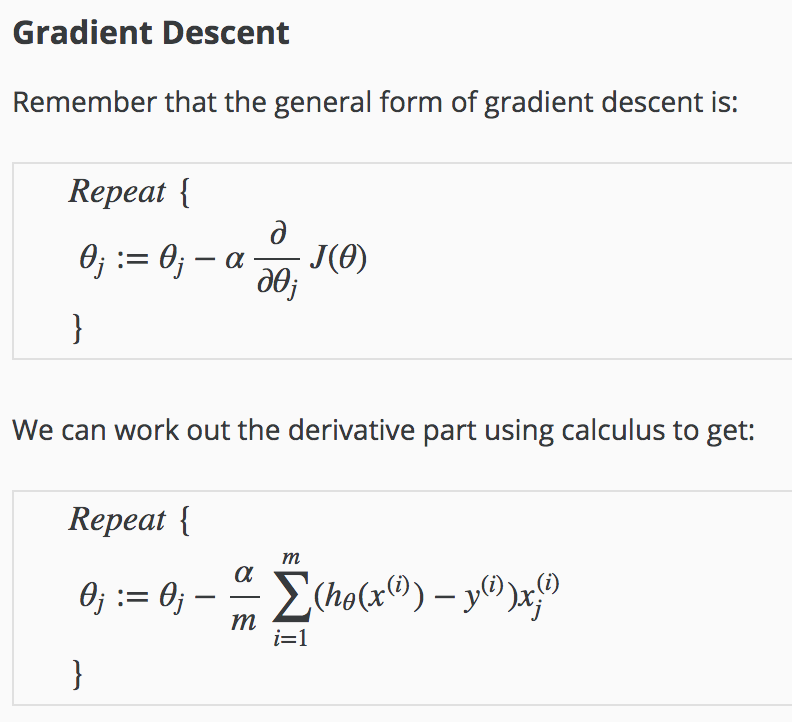
\includegraphics[scale = 0.5]{grad}
    \begin{enumerate}
        \subitem {\small 8.[c], the value after $100$ runs comes out to be $0.153$ on average}
        \subitem {\small 9.[a], the number of epochs turn out to be less than $350$}
    \end{enumerate}

\item[$\bullet$] {\bf PLA vs SGD}
    \begin{enumerate}
        \subitem {\small 10.[e]}
    \end{enumerate}

\end{enumerate}



\end{document}
